% document class
\documentclass{scrartcl}

% encoding
\usepackage[T1]{fontenc}
\usepackage[utf8]{inputenc}

% language
\usepackage[ngerman]{babel}

% math
\usepackage{amsmath}
\usepackage{amsfonts}
\usepackage{amssymb}
\usepackage{amstext}
\usepackage{isomath}
\usepackage{mathtools}

% physics
\usepackage{tensor}
\usepackage{slashed}
\usepackage{braket}
\usepackage[strict, separate-uncertainty, sticky-per]{siunitx}

% fonts
\usepackage{enumerate}
\usepackage{microtype}
\usepackage{fourier}
\usepackage{tgheros}
\usepackage{tgcursor}
\usepackage{tgpagella}

% tikz
\usepackage{tikz}

% margins
\usepackage[top=2.5cm]{geometry}

% variables
\newcommand{\thehandover}{Freitag, den 24.\,November 2017 12:00 Uhr}
\newcommand{\thesheet}{1}
\newcommand{\thesemester}{WS 17/18}
\newcommand{\theprofessor}{Priv.-Doz.~U.~Löw}

% enumeration
\renewcommand{\labelenumi}{(\alph{enumi})} % alphabetic tasks
\renewcommand{\theenumi}{(\alph{enumi})} % alphabetic tasks
\usepackage{enumitem} % allows to continue lists with [resume]

% clickable links and '\url' command
\usepackage[hidelinks]{hyperref}

% macros
\newcounter{exercise}
\newenvironment{exercise}
[2]
{\addtocounter{exercise}{1}{\bfseries{Aufgabe \arabic{exercise}:~#1}\hfill(#2 Punkte)}\newline}
{\medskip}

\setlength{\parindent}{0mm}
\begin{document}
{\large\bfseries 5. Übungsblatt zur Vorlesung\hfill\thesemester}\\
{\large\bfseries Theoretische Physik I\hfill\theprofessor}\\
{\large\bfseries Abgabe: bis \thehandover}\\
\textbf{Webseite zur Vorlesung: \\}
\url{https://moodle.tu-dortmund.de/course/view.php?id=9519}\\
\rule{\columnwidth}{0.1ex}
\medskip

\begin{exercise}{Perle auf Draht}{10}
  Betrachten Sie eine Perle auf einem Draht. Die Perle besitzt die Masse $m$
  und gleitet reibungsfrei auf einem Draht, welcher durch die Funktion $z = h(x)$
  beschrieben wird.

  \begin{figure}[h]
    \centering
    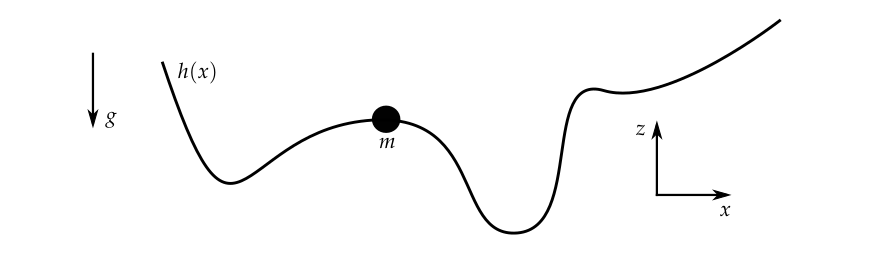
\includegraphics[width=\textwidth]{Blatt_06_PerleaufDraht.png}
    \label{fig:Höhenprofil}
  \end{figure}

    \begin{enumerate}
        \item Bestimmen Sie für einen beliebig geformten Draht $h(x)$ die Lagrange-Funktion
        in der generalisierten Koordinate $x$.
        \item Nutzen Sie die Euler-Lagrange-Gleichung, um die Bewegungsgleichung
        des Massepunktes aufzustellen.
        \item Setzen Sie nun die folgenden Funktionen $h(x)$ in die Bewegungsgleichung
        ein:
        \begin{itemize}
          \item[(i)] Welche Bewegung wird für $h(x) = h_0$ angenommen?
          \item[(ii)] $h(x) = ax$. Zeigen Sie anhand der Bewegungsgleichung, dass
          auf die Perle nur die konstante Hangabtriebskraft
          \begin{equation}
            \label{eqn:Hangabtrieb}
            \left|\vec{F}_{H}\right| = mg\sin\left(\alpha\right)
          \end{equation}
          wirkt, wobei $\alpha$ den Steigungswinkel der Funktion, d.h. den Winkel
          zwischen Funktionsgraph und der $x$-Achse, bezeichnet.
          \item[(iii)] Sei nun $h(x) = \frac{b}{2}x^2$. Die Bewegungsgleichung enthält
           neben der Hangabtriebskraft einen weiteren Term. Welche Kraft beschreibt
           dieser?\\

           Welche Form nimmt die Bewegungsgleichung für $b > 0$ an, wenn die
           Auslenkungen $x$
           und die Geschwindigkeiten $\dot{x}$ so klein sind, dass nur die linearen Terme
           berücksichtigt werden müssen?\\
         \end{itemize}
           \item Berechnen Sie aus der Lagrange-Funktion, die Sie in Aufgabenteil (a)
           bestimmt haben, die Erhaltungsgrö\ss e

    \begin{equation}
      \label{eqn:Hamilton}
      H = \dot{x}\frac{\partial L}{\partial\dot{x}} - L.
    \end{equation}
    Um welche Grö\ss e handelt es sich hierbei?
    \end{enumerate}
\end{exercise}

